\def\year{2019}\relax
\documentclass[letterpaper]{article} % DO NOT CHANGE THIS
\usepackage{aaai19}  % DO NOT CHANGE THIS
\usepackage{times}  % DO NOT CHANGE THIS
\usepackage{helvet} % DO NOT CHANGE THIS
\usepackage{courier}  % DO NOT CHANGE THIS
\usepackage[hyphens]{url}  % DO NOT CHANGE THIS
\usepackage{graphicx} % DO NOT CHANGE THIS
\urlstyle{rm} % DO NOT CHANGE THIS
\def\UrlFont{\rm}  % DO NOT CHANGE THIS
\usepackage{graphicx}  % DO NOT CHANGE THIS
\frenchspacing  % DO NOT CHANGE THIS
\setlength{\pdfpagewidth}{8.5in}  % DO NOT CHANGE THIS
\setlength{\pdfpageheight}{11in}  % DO NOT CHANGE THIS
\usepackage{amsmath}
\graphicspath{{images/}}
\nocopyright
\usepackage{array}
\usepackage{caption}
\usepackage{xcolor}
\usepackage[outputdir=output]{minted}
%PDF Info Is REQUIRED.
% For /Author, add all authors within the parentheses, separated by commas. No accents or commands.
% For /Title, add Title in Mixed Case. No accents or commands. Retain the parentheses.
\pdfinfo{
/Title (Regression)
/Author (Mark Wesley Harris)
} %Leave this	
% /Title ()
% Put your actual complete title (no codes, scripts, shortcuts, or LaTeX commands) within the parentheses in mixed case
% Leave the space between \Title and the beginning parenthesis alone
% /Author ()
% Put your actual complete list of authors (no codes, scripts, shortcuts, or LaTeX commands) within the parentheses in mixed case. 
% Each author should be only by a comma. If the name contains accents, remove them. If there are any LaTeX commands, 
% remove them. 

% DISALLOWED PACKAGES
% \usepackage{authblk} -- This package is specifically forbidden
% \usepackage{balance} -- This package is specifically forbidden
% \usepackage{caption} -- This package is specifically forbidden
% \usepackage{color (if used in text)
% \usepackage{CJK} -- This package is specifically forbidden
% \usepackage{float} -- This package is specifically forbidden
% \usepackage{flushend} -- This package is specifically forbidden
% \usepackage{fontenc} -- This package is specifically forbidden
% \usepackage{fullpage} -- This package is specifically forbidden
% \usepackage{geometry} -- This package is specifically forbidden
% \usepackage{grffile} -- This package is specifically forbidden
% \usepackage{hyperref} -- This package is specifically forbidden
% \usepackage{navigator} -- This package is specifically forbidden
% (or any other package that embeds links such as navigator or hyperref)
% \indentfirst} -- This package is specifically forbidden
% \layout} -- This package is specifically forbidden
% \multicol} -- This package is specifically forbidden
% \nameref} -- This package is specifically forbidden
% \natbib} -- This package is specifically forbidden -- use the following workaround:
% \usepackage{savetrees} -- This package is specifically forbidden
% \usepackage{setspace} -- This package is specifically forbidden
% \usepackage{stfloats} -- This package is specifically forbidden
% \usepackage{tabu} -- This package is specifically forbidden
% \usepackage{titlesec} -- This package is specifically forbidden
% \usepackage{tocbibind} -- This package is specifically forbidden
% \usepackage{ulem} -- This package is specifically forbidden
% \usepackage{wrapfig} -- This package is specifically forbidden
% DISALLOWED COMMANDS
% \nocopyright -- Your paper will not be published if you use this command
% \addtolength -- This command may not be used
% \balance -- This command may not be used
% \baselinestretch -- Your paper will not be published if you use this command
% \clearpage -- No page breaks of any kind may be used for the final version of your paper
% \columnsep -- This command may not be used
% \newpage -- No page breaks of any kind may be used for the final version of your paper
% \pagebreak -- No page breaks of any kind may be used for the final version of your paperr
% \pagestyle -- This command may not be used
% \tiny -- This is not an acceptable font size.
% \vspace{- -- No negative value may be used in proximity of a caption, figure, table, section, subsection, subsubsection, or reference
% \vskip{- -- No negative value may be used to alter spacing above or below a caption, figure, table, section, subsection, subsubsection, or reference

\setcounter{secnumdepth}{0} %May be changed to 1 or 2 if section numbers are desired.

% The file aaai19.sty is the style file for AAAI Press 
% proceedings, working notes, and technical reports.
%
\setlength\titlebox{2.5in} % If your paper contains an overfull \vbox too high warning at the beginning of the document, use this
% command to correct it. You may not alter the value below 2.5 in
\title{Regression}
%Your title must be in mixed case, not sentence case. 
% That means all verbs (including short verbs like be, is, using,and go), 
% nouns, adverbs, adjectives should be capitalized, including both words in hyphenated terms, while
% articles, conjunctions, and prepositions are lower case unless they
% directly follow a colon or long dash
\author{Mark Wesley Harris\\ % All authors must be in the same font size and format. Use \Large and \textbf to achieve this result when breaking a line
% If you have multiple authors and multiple affiliations
% use superscripts in text and roman font to identify them. For example, Sunil Issar,\textsuperscript{\rm 2} J. Scott Penberthy\textsuperscript{\rm 3} George Ferguson,\textsuperscript{\rm 4} Hans Guesgen\textsuperscript{\rm 5}. Note that the comma should be placed BEFORE the superscript for optimum readability
University of Colorado Colorado Springs\\
wharris2@uccs.edu % email address must be in roman text type, not monospace or sans serif
}
\begin{document}

\maketitle

\section{Introduction}
Regression is the process of fitting a polynomial function
to a set of data, such that predictions for unknown values can be made with some accuracy.
More specifically, regression is an optimization problem that involves minimizing errors between data
and the objective function.
%The topics discussed here, including
%Least Squares Linear Regression and Stochastic Gradient Descent,
%are important to understanding how to optimize an objective function
%for a dataset with any number of features.
Especially for noisy data,
an objective function is approximate and reflects some error
\cite{mathematical_programming}.
Thus, the regression problem arises in finding an objective function
with the least error possible for a given dataset.

\section{Least Squares Linear Regression}
Least Squares Linear Regression (LSLR) is one of the most
basic types of regression, and is widely used in practice.
The objective function for LSLR is the
minimization of loss, which is the sum
of the squares of the error between the input data vectors
and fit.
Calculation for the error of the fit is shown in Equation \ref{eq:error}.

\begin{equation}
\label{eq:error}
\epsilon^{(i)} = y^{(i)} - \hat{y}^{(i)} = y^{(i)} - \theta_0 - \sum_{j=1}^{n}(\theta_jx^{(i)}_j)
\end{equation}

The dimension of the error depends on the number of independent variables, $x_1,x_2,\dots,x_n$.
The solution for an optimization problem with $n$
independent variables will be a hyperplane of $n + 1$ dimensions.
The objective function used for LSLR is stated in Equation \ref{eq:objective_function}.
In the equation, $N$ represents the number
of true $y^{(i)}$ values, and $\epsilon^{(i)}$ is the error calculation
shown in Equation \ref{eq:error}.

\begin{equation}
\label{eq:objective_function}
\text{Find } \theta_{0},\dots,\theta_{n} \text{ such that } \mathcal{L}(\mathcal{D}) = \sum_{i=1}^{N} (\epsilon^{(i)})^2 \text{ is minimal.}
\end{equation}

%Compared to other methods of calculating loss,
%there are many benefits to minimizing the sum of the squares of error:
%\begin{enumerate}
%\item Since squared values are always positive,
%large errors do not cancel each other out. No matter if the data point is above,
%below, or on the fitted line, $\epsilon^{(i)}$ will capture the error appropriately.
%\item Using squared values produces better results than other distributions,
%since small values remain small while large values
%grow quadratically. Larger errors are thus weighted
%more heavily in this scheme, so a large $\epsilon^{(i)}$ will contribute
%more than smaller $\epsilon^{(i)}$. This behavior creates a more generalized fit.
%\item Finally, the sum of the squares of error is mathematically trivial to
%derive, and thus finding the minimum is doable in constant time.
%This is expressed as
%$$\frac{d}{d\theta_0}\mathcal{L} =
%\sum_{i=1}^{N}(y^{i} - \theta_0 - \theta_1x^{i})$$
%$$\frac{d}{d\theta_1}\mathcal{L} =
%x^{(i)}\sum_{i=1}^{N}(y^{i} - \theta_0 - \theta_1x^{i})$$
%By setting these derivatives equal to 0 and plugging in
%$x_1,x_2\dots,x_n$, we may find the minimum of the linear equation.
%\end{enumerate}

\section{Stochastic Gradient Descent}
The basic principle behind gradient descent is shown in Figure \ref{fig:machine_learning}.
Gradient descent involves calculating
a value along the negative gradient of an objective function, in order to approximate
the minimum.
%The process of approximation is important;
%if the step of the descent is too large, the minimum may not be reached,
%but if the step is too small it will take a significant amount time to find it
%or become trapped in local minima.
%The gradient step must be chosen carefully in order to provide good
%results in a reasonable amount of time.
The gradient represents the direction (in terms of each feature)
for how fast a function is approaching the maximum at a given point.
Thus, the solution for the objective function
can be approximated using the gradient, as is shown in Equation \ref{eq:gradient}.
In order to ensure a shorter time taken for each iteration,
the concept of using batches was introduced.
A batch is a subset of the entire dataset \cite{machine_learning}.

\begin{equation}
\label{eq:gradient}
\nabla \mathcal{L} = \sum_{i=1}^{n}\frac{\partial \mathcal{L}}{\partial \theta_i} = -2\theta_0(\epsilon^{(i)}) - 2x^{(i)}(\epsilon^{(i)})
\end{equation}

\begin{figure}[htbp]
\centerline{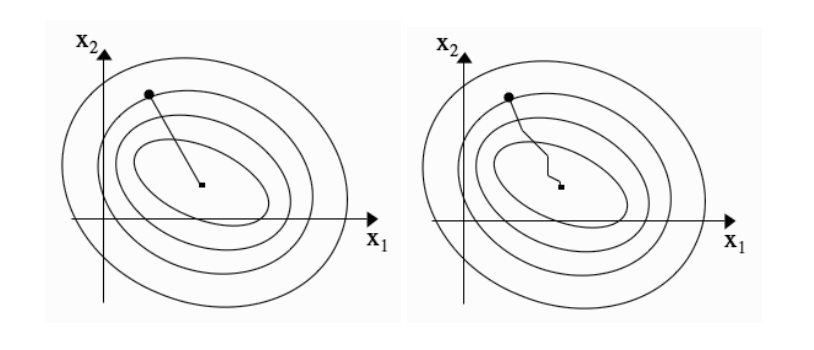
\includegraphics[width=8cm]{machine_learning.png}}
\caption{Ideally, the minimum would be reached directly (left).
However in practice, it is more feasible to obtain the solutions through approximation (right)
\cite{machine_learning}.}
\label{fig:machine_learning}
\end{figure}

Stochastic Gradient Descent (SGD) is a special type of gradient descent,
where each batch is comprised of one input vector chosen at random.
The algorithm iteratively tries to find the global minimum
by updating each coefficient by a factor of the negative gradient.
SGD uses the formula in Equation \ref{eq:gradient} along with a learning parameter, $\lambda$,
to iteratively find the coefficients $\theta_{0},\dots,\theta_{n}$ that give the
minimum error possible.
In practice, $\lambda$ must be not so high as to lose the benefit from previous generations,
but also not so low as to disregard the impact of the current iteration.
The update for each coefficient, $\theta_i$, is given in Equation \ref{eq:sgd}.

\begin{equation}
\label{eq:sgd}
\theta_i = \theta_i - \lambda \nabla \mathcal{L}
\end{equation}

Stochastic Gradient Descent is thoroughly studied, and research shows many
theoretical and practical motivations behind using SGD
\cite{large-scale_optimization}.
Compared to other optimization algorithms,
SGD is less likely to get stuck at
local minima,
and on average requires less time to run.
SGD is often used to optimize nueral networks, however
gradient-free algorithms can be advantageous
when dealing with a
``\dots complex and poorly-understood optimization landscape''
\cite{evolutionary_sgd}.
SGD is also also often used if the training dataset is very large, since
in that case
``\dots it would be very expensive to use the whole dataset to estimate
the gradient'' \cite{machine_learning}.

\section{Implementation}
All code was written in Python, using the numpy and pandas
libraries for processing input data.
An overview of the implementation for SGD involved the following:

\begin{enumerate}
\item Initialize the coefficients to some random or guess value.
\item Iterate over a set of data.
\item In each iteration, update the coefficients based off Equation \ref{eq:sgd}.
\end{enumerate}

Implementing SGD for Ridge Regression only involved a simple change to the
gradient function in the form of an extra parameter, $\alpha$.
The updated gradient equation is shown in Equation \ref{eq:ridge}.
For simplicity, it was decided to use this equation for LSLR as well,
but set $\alpha$ equal to 0.

\begin{equation}
\label{eq:ridge}
\nabla \mathcal{L} = -2\theta_0(\epsilon^{(i)}) - 2x^{(i)}(\epsilon^{(i)}) + 2\alpha x^{(i)}
\end{equation}

Several regression solutions in existing libraries were used in order to compare the fits
produced by the SGD method.
Models for LSLR, Ridge, Lasso, and Elastic Net
were implemented using the sklearn Python library.
The Lasso Regression and Elastic Net Regression models
were run on non-normalized data in order to produce non-zero $R^2$ values.
Thus, we can still compare their effectiveness to the other implementations,
however the coefficients are scaled differently.
Evaulations for each model are included in Table \ref{tbl:goodness},
and the loss for each distribution is shown in Figures \ref{fig:my_evaluation} and \ref{fig:lib_evaluation}.


\section{Dataset}
The Combined Cycle Power Plant dataset
found in the UCI Machine Learning Repository was used to test the implementations.
The first few rows of the CCPP dataset are given in
Table \ref{tbl:ccpp}.
The dataset represents a distribution for energy output ($PE$),
which is based on the features of
average temperature ($AT$),
exhaust vacuum ($V$),
ambient pressure ($AP$),
and relative humidity ($RH$).
Thus, the optimization problem presented is to predict $PE$ given
values for $AT$, $V$, $AP$, and $RH$.

\begin{table}[t]
\begin{centering}
\bgroup
\def\arraystretch{1.5}
\begin{tabular}{| m{0.07\textwidth} | m{0.07\textwidth} | m{0.07\textwidth} | m{0.07\textwidth} | m{0.07\textwidth}|} 
\hline
$AT$ & $V$ & $AP$ & $RH$ & $PE$ \\ 
\hline
\hline
14.96 & 41.76 & 1024.07 & 73.17 & 463.26 \\ 
\hline
25.18 & 62.96 & 1020.04 & 59.08 & 444.37 \\ 
\hline
\ldots & \ldots & \ldots & \ldots & \ldots \\ 
\hline
\end{tabular}
\caption{Samples from the CCPP dataset.}
\label{tbl:ccpp}
\egroup
\end{centering}
\end{table}

It was found through testing that $\lambda = 0.1$ gave good results
for both LSLR and Ridge Regression.
Further experiments were done in order to find the optimal value of $\alpha$
for Ridge Regression. It was found that any value greater than 0.1 resulted
in worse learning for the model, represented by lower $R^2$ values.
$\alpha = 0$ gave the best $R^2$ value, 
however since this results in the same gradient as LSLR,
the value of $\alpha = 0.1$ was chosen for comparison of the two models.

Figure \ref{fig:loss_per_epoch} shows a comparison how well the implementations of LSLR and Ridge Regression
minimized error for the CCPP dataset throughout the course of learning.
Both models in general decrease loss in each sequential epoch,
which shows how the SGD alogrithm slowly obtains optimal values
for $\theta_{0},\dots,\theta_{n}$ as the number of iterations increases.
It is also clear from the graph that LSLR faired better overall
and ended with a better fit.
A total of 15,000 epochs were run for each model, which was found to better the overall fit for both models.

\begin{figure}[htbp]
\centerline{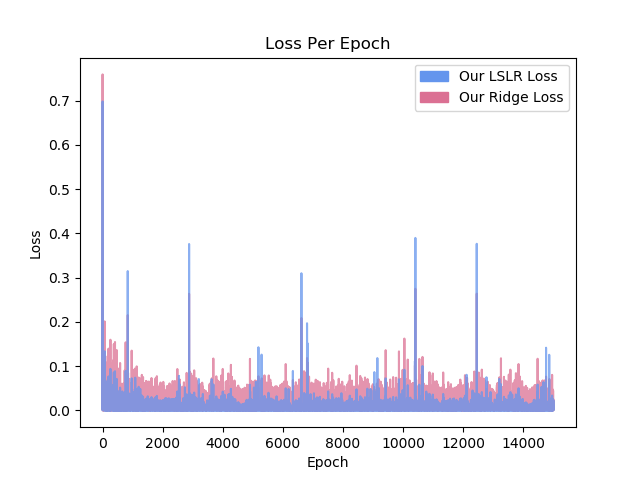
\includegraphics[width=10cm]{loss_per_epoch.png}}
\caption{Loss ($\epsilon = (y^{(i)} - \hat{y}^{(i)})^2$) per epoch of SGD.}
\label{fig:loss_per_epoch}
\end{figure}

\section{Results}
The final fits calculated for each model are shown in Table \ref{tbl:fits}.
The fits for our LSLR and Ridge Regression implementations
are very close to the fits of the library implementations.
However, we must also keep in mind that since SGD uses randomness in order to optimize the objective function,
the algorithms generate slightly different coefficients on each run.
The library implementations are not only repeatable, but also take less time
to calculate.
The Lasso Regression and Elastic Net Regression models only produced
good fits (an $R^2$ above 0) when the dataset was normalized.
This is why there is a significant difference in the fits for the models
shown in Table \ref{tbl:fits} compared to the fits for LSLR and Ridge Regression.

\begin{table}[t]
\begin{centering}
\bgroup
\def\arraystretch{1.5}
\begin{tabular}{| m{0.07\textwidth} | m{0.355\textwidth} |} 
\hline
Method & Fit \\ 
\hline
\hline
Our LSLR & $1.10230 - 0.93027AT - 0.15797V + 0.04194AP - 0.14884RH$ \\
\hline
Our Ridge & $1.05230 - 0.93026AT - 0.15797V + 0.04194AP - 0.14884RH$ \\
\hline
LSLR & $1.09191 - 0.92459AT - 0.17412V + 0.03323AP - 0.15617RH$ \\
\hline
Ridge & $1.08467 - 0.91278AT - 0.18085V + 0.03676AP - 0.15154RH$ \\
\hline
Lasso* & $466.54407 - 1.92235AT - 0.25197V + 0.04907AP - 0.14247RH$ \\
\hline
Elastic Net* & $435.71149 - 1.85600AT - 0.27840V + 0.07906AP - 0.13452RH$ \\
\hline
\end{tabular}
\caption{Enumeration of fit for each model. Models marked with an asterisk
were non-normalized.}
\label{tbl:fits}
\egroup
\end{centering}
\end{table}

\section{Evaluation and Goodness of Fit}
One way to evaluate the models is to meausre the losses of the
fit over the dataset. These results are shown in Figure \ref{fig:my_evaluation}
and Table \ref{tbl:goodness}.
LSLR has generally lower losses than Ridge Regression,
while Lasso and Elastic Net gave higher means.
This implies that for any given point in the dataset they produce higher loss
than the LSLR or Ridge Regression models.

$R^2$ is another way to evaluate the effectiveness of a model.
The $R^2$ value compares the loss of the fit with that of the data.
Equation \ref{eq:r-squared} was used to calculate $R^2$.
$\overline{y}$ denotes the mean of the real data,
$SSE$ represents loss of the fit itself,
and $SST$ represents total loss within the dataset.
The calculated values for each model can be found in Table \ref{tbl:goodness} beside the mean losses.
An $R^2$ close to 1 shows a good fit, meaning all the models achieved fairly good results.

\begin{equation}
\label{eq:r-squared}
R^2 = 1 - \frac{SSE}{SST} = \frac{\sum_{i=1}^{N}(y^{(i)} - \hat{y}^{(i)})^2}{\sum_{i=1}^{N}(y^{(i)} - \overline{y})^2}
\end{equation}

The $p$-value is another measurement of goodness of fit.
We attempted to find $p$-values for the LSLR and Ridge Regression
implementations as well as for the libraries; however,
the $p$-values were either exceptionally low (nearly 0) or
exceptionally high (approching 1).
This could be in part due to the normalization of data
or the number of entries in the dataset;
as the number of cells in a table increases
``\dots in multivariate discrete data analysis, most often,
the $p$-values for these statistics cannot be trusted'' \cite{goodness}.
The $p$-values were disregaurded as measures of goodness of fit for this dataset.

\begin{table}[t]
\begin{centering}
\bgroup
\def\arraystretch{1.5}
\begin{tabular}{| m{0.06\textwidth} | m{0.17\textwidth} | m{0.17\textwidth}|} 
\hline
Method & $R^2$ & Mean Loss for Fit \\ 
\hline
\hline
Our LSLR & 0.916392457 & 0.003693939 \\
\hline
Our Ridge & 0.916232524 & 0.014153592 \\
\hline
LSLR & 0.928696089 & 0.003643243 \\
\hline
Ridge & 0.928696089 & 0.003644301 \\
\hline
Lasso & 0.928185843 & 0.051094579 \\
\hline
Elastic Net & 0.928185843 & 0.051094579 \\
\hline
\end{tabular}
\caption{Evaluation for the goodness of fit.}
\label{tbl:goodness}
\egroup
\end{centering}
\end{table}

\begin{figure*}[htbp]
\centerline{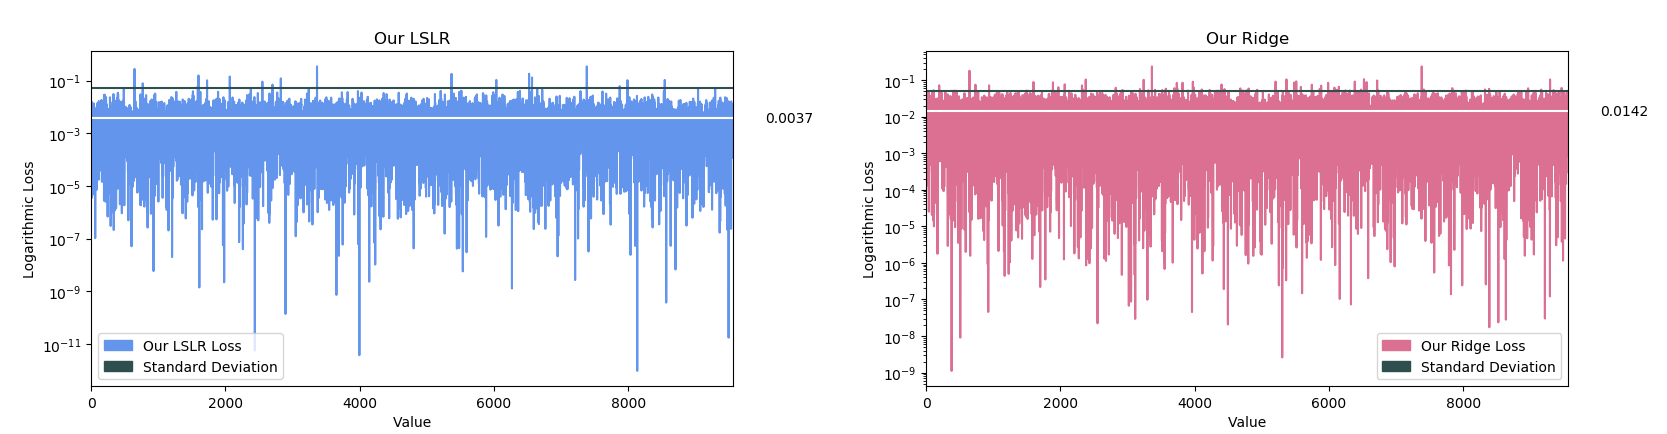
\includegraphics[width=\textwidth]{my_evaluation.png}}
\caption{Logarithmic loss ($\epsilon = (y^{(i)} - \hat{y}^{(i)})^2$) for 15,000 epochs using
$\lambda = 10^{-2}$ (LSLR and Ridge) and $\alpha = 10^{-2}$ (Ridge).
The mean of loss is shown using a white line and value to the right of each plot.
Means are also shown in Table \ref{tbl:goodness}.}
\label{fig:my_evaluation}
\end{figure*}

\begin{figure*}[htbp]
\centerline{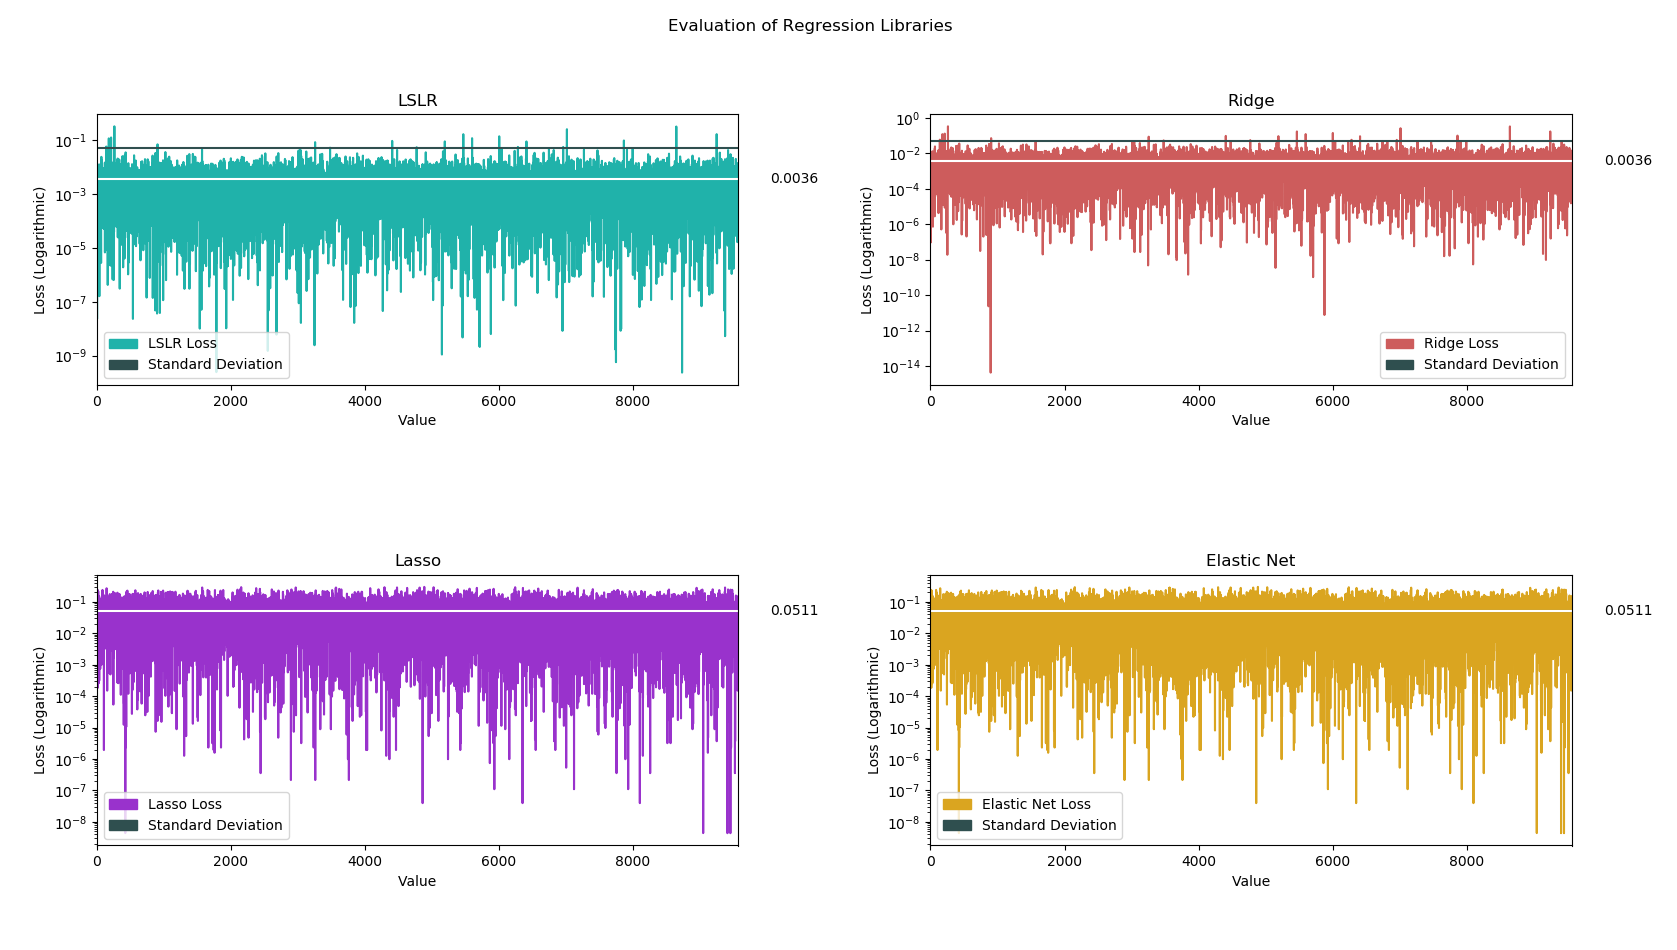
\includegraphics[width=\textwidth]{lib_evaluation.png}}
\caption{Comparison of logarithmic loss ($\epsilon = (y^{(i)} - \hat{y}^{(i)})^2$) for regression
solutions of existing libraries.
The mean of loss is shown using a white line and value to the right of each plot.
LSLR had the lowest mean loss, with a difference between Ridge Regression of
$1.05848*10^{-6}$.}
\label{fig:lib_evaluation}
\end{figure*}

\section{Conclusion}
We found that out of the two regression models implemented using Stochastic Gradient Descent,
LSLR produced the best fit. Even out of the implementations found in the libraries,
LSLR had the lowest mean loss and highest $R^2$ value.
Although none of the $R^2$ values dropped below 0.9,
there was a notable difference in the quality of fit for the
Lasso Regression and Elastic Net Regression models.
We can assume from this that allowing some of the coefficients to drop completely to zero
was not completely representative of the fit for the entire dataset.
SGD was found to be less reliable than the methods implemented in standard libraries,
however it can still give good results depending on the problem to which it is applied.

\nocite{large_scale}
\nocite{overview_optimization}
\nocite{intro_sgd}

\bibliography{report}
\bibliographystyle{aaai}

\onecolumn

\pagebreak

\begin{center}
\section*{Appendix}
\label{app:b}
\end{center}

\bigskip

\footnotesize{
\begin{minted}{python}
# sgd.py

import pandas as pd
import numpy as np

# Definition of Stochastic Gradient Descent algorithm.
def sgd(data, coeffs, alpha, beta):
    # Setup y and y_hat.
    row = [1, data['AT'], data['V'], data['AP'], data['RH']]
    y_real = data['PE']
    y_pred = np.dot(row, coeffs)

    # Calculate next values.
    for i in range(0, len(row)):
        coeffs[i] = coeffs[i] - alpha * gradient(i, row[i], y_real, y_pred, beta)

    return coeffs, y_real, y_pred

# Definition for approximating the gradient of the objective function.
def gradient(i, x, y_real, y_pred, alpha):
    if i > 0:
        return (-2 * x * (y_real - y_pred)) + (2 * alpha * x)
    else:
        return (-2 * (y_real - y_pred)) + (2 * alpha * x)
\end{minted}
\bigskip
\begin{minted}{python}
# utilities.py

import pandas as pd
import numpy as np
import random
import matplotlib.pyplot as plt
import matplotlib.patches as mpatches
from sklearn.utils import shuffle
from scipy.stats import ttest_1samp
from scipy.stats import ttest_ind
from scipy.stats import ttest_rel
from scipy.stats import f_oneway

#Function for importing CCPP dataset.
def import_CCPP(normalize):
    dataset = pd.read_excel('./source/CCPP/Folds5x2_pp.xlsx')
    dataset = shuffle(dataset)
    dataset.reset_index(inplace=True, drop=True)
    if normalize:
        dataset = (dataset - dataset.min())/(dataset.max() - dataset.min())
    return dataset

# Function for returning a random row of a dataset.
def random_row(dataset):
    index = random.randint(0, len(dataset.index) - 1)
    return dataset.iloc[index,:]

# Define loss function.
def loss(a, b):
    return (a - b) ** 2

# Definition for Squared Sum of Errors.
def SSE(dataset, coeffs):
    sse = 0
    for index, data in dataset.iterrows():
        y_real = data['PE']
        row = [1, data['AT'], data['V'], data['AP'], data['RH']]
        y_pred = np.dot(coeffs, row)

        sse += (y_real - y_pred) ** 2

    return sse

# Definition for Squared Sum of Total Error.
def SST(dataset, coeffs):
    sst = 0
    y_mean = np.mean(dataset.iloc[:,4].values)
    for index, data in dataset.iterrows():
        y_real = data['PE']

        sst += (y_real - y_mean) ** 2

    return sst

# Definition for R^2.
def R_squared(dataset, coeffs):
    return (1 - SSE(dataset, coeffs) / SST(dataset, coeffs))

def T_test(dataset, coeffs):
    y_real = np.array(dataset.iloc[:,4].values)
    y_pred = []
    for index, data in dataset.iterrows():
        row = [1, data['AT'], data['V'], data['AP'], data['RH']]
        pe_pred = np.dot(coeffs, row)
        y_pred.append(pe_pred)

    y_pred = np.array(y_pred)

    print(ttest_ind(y_pred, y_real))
    print(ttest_ind(y_pred, y_real, equal_var=False))
    print(ttest_rel(y_pred, y_real))
    print(f_oneway(y_pred, y_real))

# Definition for overall statistics function.
def stats(dataset, fit, title, normalized):
    print('Stats For ' + title + ':')
    T_test(dataset, fit)
    print('Fit:       ', fit)
    print('R-squared: ', R_squared(dataset, fit))
    print('\n')

# Definition for plotting loss values, for two-dimensional case.
def plot_loss(epochs, losses, dataset, title, color):
    x_axis = np.linspace(0, epochs, len(losses), endpoint=True)
    plt.semilogy(x_axis, losses, color=color)

    # Line at loss = std(y)^2.
    y_real = dataset.iloc[:,4].values
    plt.axhline(y=np.std(y_real)**2, color='darkslategray', xmin=0,
                xmax=epochs, linestyle='-')

    loss_patch = mpatches.Patch(color=color)
    std_patch = mpatches.Patch(color='darkslategray')
    plt.legend([loss_patch, std_patch], ['Loss', 'Standard Deviation'])
    plt.xlabel('Epoch')
    plt.ylabel('Logarithmic Loss')
    plt.title(title)
    plt.show()

# Definition for plotting loss values, for two-dimensional case.
def plot_fit(dataset, coeffs, title, color):
    losses = []
    y_real = np.array(dataset.iloc[:,4].values)
    for index, data in dataset.iterrows():
        row = [1, data['AT'], data['V'], data['AP'], data['RH']]
        y_pred = np.dot(coeffs, row)
        losses.append(loss(y_real[index], y_pred))

    x_axis = np.linspace(0, len(dataset.iloc[:,4].values), len(losses), endpoint=True)
    plt.plot(x_axis, losses, color=color)
    plt.xlim(0, len(dataset.iloc[:,4].values))

    # Line at loss = std(y)^2.
    plt.axhline(y=np.std(y_real)**2, color='darkslategray', xmin=0,
                xmax=len(dataset.iloc[:,4].values), linestyle='-')

    loss_patch = mpatches.Patch(color=color)
    std_patch = mpatches.Patch(color='darkslategray')
    plt.legend([loss_patch, std_patch], ['Loss', 'Standard Deviation'])
    plt.xlabel('Value')
    plt.ylabel('Logarithmic Loss')
    plt.title(title)
    plt.show()
\end{minted}
\bigskip
\begin{minted}{python}
# my_lslr.py
import pandas as pd
import numpy as np
import random
import utilities
from sgd import sgd

# Definition of Least Squares Linear Regression algorithm.
def my_lslr(dataset, max_epochs, alpha):
    # Initialize local variables
    coeffs = [0.0 for i in range(len(dataset.iloc[0,:]))]
    losses = []
    epochs = 0

    # Iterate over the dataset until max epochs has been reached.
    while epochs < max_epochs:
        for index, data in dataset.iterrows():
            # Run the SGD algorithm.
            coeffs, y_real, y_pred = sgd(data, coeffs, alpha, 0)

            # Record loss for this epoch.
            losses.append(utilities.loss(y_real, y_pred))

            # Stop conditions.
            epochs += 1
            if epochs >= max_epochs:
                break

    print(epochs)
    return coeffs, losses
\end{minted}
\bigskip
\begin{minted}{python}
# lslr.py

import pandas as pd
import numpy as np
from sklearn.linear_model import LinearRegression
import utilities

# Definition of Least Squares Linear Regression algorithm.
def lslr(dataset):
    # Initialize local variables
    x = dataset.iloc[:,0:4].values
    y = dataset.iloc[:,4].values

    regressor = LinearRegression()
    regressor.fit(x, y) #training the algorithm

    return np.append(regressor.intercept_, regressor.coef_)
\end{minted}
\bigskip
\begin{minted}{python}
# ridge.py

import pandas as pd
import numpy as np
from sklearn.linear_model import Ridge
import utilities

# Definition of Ridge Regression algorithm.
def ridge(dataset):
    # Initialize local variables
    x = dataset.iloc[:,0:4].values
    y = dataset.iloc[:,4].values

    regressor = Ridge()
    regressor.fit(x, y) #training the algorithm

    return np.append(regressor.intercept_, regressor.coef_)
\end{minted}
\bigskip
\begin{minted}{python}
# lasso.py

import pandas as pd
import numpy as np
from sklearn.linear_model import Lasso
import utilities

# Definition of Lasso Regression algorithm.
def lasso(dataset):
    # Initialize local variables
    x = dataset.iloc[:,0:4].values
    y = dataset.iloc[:,4].values

    regressor = Lasso()
    regressor.fit(x, y) #training the algorithm

    return np.append(regressor.intercept_, regressor.coef_)
\end{minted}
\bigskip
\begin{minted}{python}
# elastic.py

import pandas as pd
import numpy as np
from sklearn.linear_model import ElasticNet
import utilities

# Definition of Elastic Net Regression algorithm.
def elastic(dataset):
    # Initialize local variables
    x = dataset.iloc[:,0:4].values
    y = dataset.iloc[:,4].values

    regressor = ElasticNet()
    regressor.fit(x, y) #training the algorithm

    return np.append(regressor.intercept_, regressor.coef_)
\end{minted}
}

\end{document}
